\item{processes of ranking}
Actually, there are 4 missions for the whole championship, and every mission has different rules and penalties, but the processes of every mission works similarly, when a team finished an attempt, we should create a score for this attempt, from the algorithm we used, we could get the time cost or a raw score differed from missions. Here I take an example of triangular course to illustrate the process to obtain the best score, where Hi means human intervention:
\begin{figure}[h!]
\centering
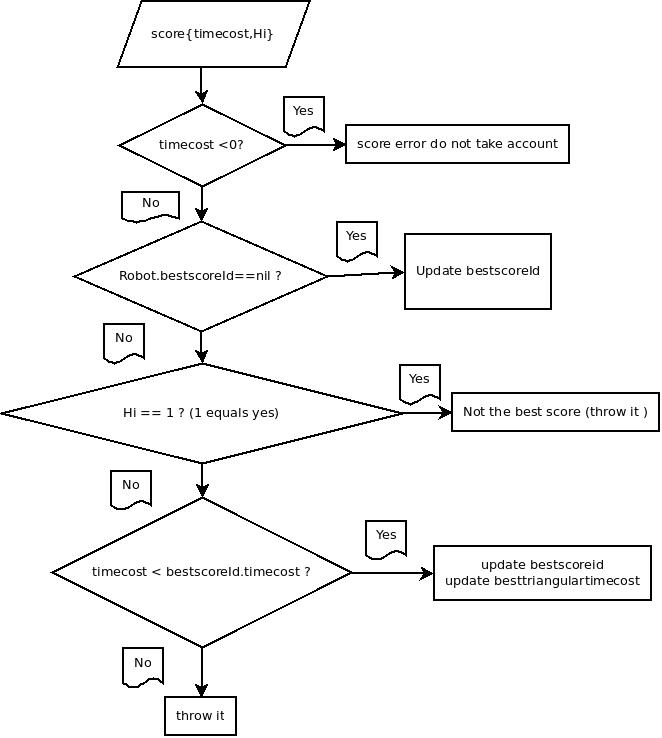
\includegraphics[width=15cm]{triangular.jpg}
\caption{new sign in }
\label{fig-sample}
\end{figure}
After obtaining the best score for every team, we could calculate the rank. Here something should be noticed, the AIS points are not taken into account in every single mission, but in the final score, we should add the AIS points.

